\documentclass[12pt,a4paper]{article}
\usepackage[a4paper, left=0.8in, right=0.8in, top=0.5in, bottom=1in]{geometry}
\usepackage[utf8]{inputenc}
\usepackage{listings}
\usepackage[hidelinks]{hyperref}
% \usepackage{gvv}
% \usepackage{gvv-book}
\usepackage{graphicx}
\graphicspath{ {./Figures/} }
\usepackage{amsmath}
\usepackage{tabularx}
\usepackage{amsfonts}
\usepackage{amssymb}
\usepackage{titlesec}

\let\vec\mathbf

% Customizing section and subsection fonts
\titleformat{\section}{\large\bfseries}{\thesection}{1em}{}
\titleformat{\subsection}{\normalsize\bfseries}{\thesubsection}{1em}{}
\renewcommand{\abstractname}{\hfill Abstract \hfill}

\title{Software Assignment: Implementing and Optimizing Eigenvalue Calculation for Arbitrary Square Matrices}
\author{Shiven Bajpai\\\small AI24BTECH11030}
\date{\today}

\begin{document}

\maketitle

\begin{abstract}
\textit{This report details the exploration and implementation of a program to compute the eigenvalues of arbitrary square matrices. Various algorithms are discussed and a couple techniques are evaluated, but the primary focus is on optimization and performance improvements. The report also discusses supporting complex eigenvalues.}
\end{abstract}

% \tableofcontents

\section{Introduction}

Eigenvalues and eigenvectors are fundamental in linear algebra and play a crucial role in various scientific and engineering applications. While eigenvectors can be easily found by solving a system of linear equations if you know the eigenvalues, determining eigenvalues for matrices larger than $4\times4$ \footnote{The Abel-Ruffini theorem proves the impossibility of a general deterministic solution for such polynomials with degree greater than 4.} is significantly more challenging. For an $n\times n$ matrix, the problem involves solving a polynomial equation of degree $n$, which becomes computationally very complicated and difficult for large $n$.
\\

However, for certain special types of matrices, eigenvalues are immediately available. Particularly, in Diagonal Matrices and Triangular Matrices, The eigenvalues are the elements of the principal diagonal.
\\

Given the complexity of direct computation, most methods aim to transform a matrix into a triangular matrix while preserving its eigenvalues. Unfortunately, operations like row reduction alter the eigenvalues, so they cannot be used directly. Instead, many algorithms rely on finding \textbf{similar matrices} of triangular form through iterative approaches, which retain the same eigenvalues but represent the transformation in a different basis.
\\

More specifically, the algorithms iterate towards a an approximation of a triangular matrix called a Hessenberg matrix, Where all elements below the principal diagonal are 0. For Hermitian matrices, certain algorithms like Lanczos produce a tridiagonal form as a special case.
\\


\section{A Summarization of Algorithms Considered}

There are plethora of different algorithms for the purpose of finding eigenvalues. Some of these are listed below
{
\renewcommand{\arraystretch}{1.6}
\begin{center}
    \begin{tabularx}{\textwidth}{| X | X |}
        \hline
        \multicolumn{1}{|c|}{Name} & \multicolumn{1}{|c|}{Description} \\
        \hline
        Arnoldi Iteration & The Arnoldi Iteration is an iterative algorithm used to compute a few eigenvalues and corresponding eigenvectors of a large square matrix. It is particularly effective for sparse or structured matrices\\  
        \hline
        Lanczos Algorithm & An much more optimized form of Arnoldi Iteration that applies only to Hermitian matrices.\\  
        \hline
        Power Iteration/ Von Mises Iteration & Iteratively finds the largest eigenvalue and corresponding Eigenvector \\
        \hline
        Inverse Iteration & Allows one to find an Eigenpair with value closest to some initial approximation\\  
        \hline
        QR Factorization & Uses repeated QR factorization to form a similar Hessenberg matrix that allows us to get all the eigenvalues, Explained in greater detail in the next subsection\\  
        \hline
        Divide and Conquer & Involves recursively dividing a matrix into smaller matrices which are then solved for their eigenvalues, These results are then combined with rank 1 (or in some cases) rank 2 corrections for the subdiagonal elements lost when dividing the matrix into smaller parts. Very fast, but more applicable to sparse matrices or other special cases as it requires a tridiagonal matrix to start off\\  
        \hline
        Jacobi Algorithm & Uses Givens rotations to iterate towards an approximation of a diagonal matrix.\\  
        \hline
        Homotopy Method & Exploits the continous change of eigenvalues when a smooth transformation is applied. By "homotoping" a simple matrix with known eigenvalues to the target matrix, we can approximate its eigenvalues. Very dependent on picking the right known matrix and path \\    
        \hline
        Automatic Multi-level Substructuring \newline (AMLS) & A more recent technique developed by U.Texas that is designed for very large sparse matrices. Although It sees use in certain simulation and engineering problems, It is not useful as a general algorithm\\
        \hline
    \end{tabularx}
\end{center}}

\subsection{QR Factorization}

The QR algorithm was created in the late 1950s and was one of the most significant algorithms of the 20th century. The algorithm goes as follows:

\begin{enumerate}
    \item \textbf{Start with a matrix \( \vec{A_0} \)}:
    Set \( \vec{A_0} = \vec{A} \), where \( \vec{A} \) is the matrix whose eigenvalues are to be computed.

    \item \textbf{Perform the QR decomposition:}
    At each iteration \( k \), decompose the matrix \( \vec{A_k} \) into the product of an orthogonal matrix \( \vec{Q_k} \) and an upper triangular matrix \( \vec{R_k} \):
    \begin{align}
        \vec{A_k} = \vec{Q_k} \vec{R_k}.
    \end{align}

    \item \textbf{Update the matrix:} Form the next matrix in the sequence by multiplying \( \vec{R_k} \) and \( \vec{Q_k} \) in reverse order:
    \begin{align}
        \vec{A_{k+1}} = \vec{R_k} \vec{Q_k}.
    \end{align}

    \item \textbf{Repeat until convergence:} The sequence of matrices \( \{\vec{A_k}\} \) converges to a matrix that is close to upper triangular form (Hessenberg Matrix):
    \begin{align}
    \vec{A_k} \to \vec{T},
    \end{align}

    where \( \vec{T} \) is an upper triangular matrix. The eigenvalues of \( \vec{A} \) are then approximately the diagonal entries of \( \vec{T} \).
\end{enumerate}

\noindent This works because the final matrix \( \vec{A}_k \) is similar to the initial matrix. Proof:

\begin{align}
    \vec{A}_k &= \vec{R}_{k-1} \vec{Q}_{k-1}\\
    \vec{A}_k &= \vec{Q}_{k-1}^\text{T} \vec{A}_{k-1} \vec{Q}_{k-1}\\
    \vec{A}_k &= \vec{Q}_{k-1}^\text{T} \vec{Q}_{k-2}^\text{T} \vec{A}_{k-2} \vec{Q}_{k-2} \vec{Q}_{k-1}\\
    \vec{Q} &= \vec{Q}_0 \vec{Q}_1 \cdots \vec{Q}_{k-1} \ \ \ \text{(Let)} \\
    \vec{A}_k &= (\vec{Q})^\text{T} \vec{A}_0 \vec{Q} \label{similarity equation}
\end{align}

\noindent Since Matrices $\vec{Q}_i$ are all orthonormal, $\vec{Q}$ is also orthonormal. Thus we can say that \eqref{similarity equation} is a similarity relation where $\vec{Q}$ serves as the change of basis matrix.
$\therefore \vec{A}_k$ is similar to $\vec{A}_0$

\subsection{Why QR is preferred}

QR has multiple advantage over the other approaches. While certain algorithms may be faster for specific cases. QR is directly applicable to ALL matrices and gives reasonably good performance in all cases.

\section{Approaches to QR}

\subsection{Gram-Schmidt Process}

Perhaps the easiest approach to implement. It involves orthogonalizing the columns of $\vec{A}$ by subtracting the projections of one column on every previous column from itself to produce $\vec{Q}$. $\vec{R}$ is simultaneously calculated to ensure that the matrix product $\vec{QR}$ gives $\vec{A}$.

\subsection{Householder Reflections}

For each column, we take the current values and the desired values, and compute a transformation called the Householder Reflection/Householder Transformation which reflects it about some hyperplane to give us the desired vector. For the $i^{th}$ column we ignore previous columns and we also ignore $i$ rows from the top, calculating Householder transformations only for the $n-i \times n-i$ submatrix left (assuming a matrix of size $n \times n$). We then extend the computed transformation to size $n \times n$ by simply padding with to the left and top and setting the new diagonal elements to 1.

\subsection{Givens Rotations}

This algorithm works by applying a series of rotations that zero out each individual element we want to change to zero. This is highly inefficient for dense matrices, and mainly shines for sparse matrices where along with a few other Optimizations, it can greatly reduce the number of operations required. However due to its poor applicability to general dense matrices, I have not implemented it here.

\subsection{A note on Numerical Stability}

Although Gram-Schmidt is simpler than and as this report will show, in many cases faster than Householder, It involves a repeated subtractions which can lead to rounding errors which can add up over time. This means that the orthogonal matrix $\vec{Q}$ might slightly deviate from orthongonality, $\vec{QQ}^\text{T}\ne\vec{I}$ but rather a very close approximation of $\vec{I}$. In householder however, since subsequent transformations don't affect previous ones and there is limited addition/subtraction, Orthogonality better. This can be remedied by re-orthogonalizing in Gram-Schmidt at every step but that affects performance poorly.
\\

Nonetheless, both give accurate eigenvalues upto many decimal places, which is good enough for most basic purposes.

\section{Generalizing to Complex Numbers}

Supporting complex numbers is a relatively straightforward process. It involves 2 parts

\begin{enumerate}
    \item \textbf{Handling Complex Matrix Elements:} This is relatively simple. We adjust our certain operations like the calculation of absolute value and square root to perform the right calculations for complex numbers.
    
    \item \textbf{Handling Complex Eigenvalues:} When we converge the matrix to to the Hessenberg form, Instead of approximating an upper triangular matrix, It forms a Quasi-Triangular matrix wherein the elements on the diagonals are made up of $1 \times 1$ or $2 \times 2$ blocks. The real eigenvalues are simply the value in the $1 \times 1$ block whereas the complex eigenvalues are gotten by solving for the eigenvalues of the $2 \times 2$ blocks. This can be done easily by solving the quadratic characteristic equation. I found that sometimes these $2 \times 2$ share a common corner, In which case solving one in place, substituting back the eigenvalue on the diagonal and then using that when solving the other block gave the right eigenvalues.
\end{enumerate}

\section{Time complexity}

\subsection{Gram-Schmidt}

Let $n$ denote the number of rows and of columns of $\vec{A}$. For each column $i$, the Gram-Schmidt process involves the following operations:
\begin{enumerate}
    \item Compute the projections with every column $j$ for $j = 1, 2, \ldots, i-1$ and subtract it, both of which are $O(n)$ operations. Thus, each projection has a cost of $O(n)$, and there are $(i-1)$ such projections for column $i$.
\end{enumerate}

The total work for column $i$ is therefore:
\[
O((i-1) \cdot n + n) = O(i \cdot n).
\]

Summing over all $n$ columns, the total cost of the Gram-Schmidt process per QR Factorization is:
\[
\sum_{i=1}^{n} O(i \cdot n) = O(n \cdot \sum_{i=1}^{n} i) = O(n^3).
\]

\subsection{Householder Reflections}

To analyze the time complexity, consider the operations involved for each column:
\begin{enumerate}
    \item Construction of \( v \): This involves computing the norm of a sub-vector of length \( n-i+1 \), which requires \( O(n-i+1) \) operations.
    \item Matrix-vector multiplication \( v^T A \): Each transformation requires a matrix-vector multiplication involving a submatrix of size \( (n-i+1) \times n \). This step costs \( O((n-i+1) \cdot n) \).
    \item Applying the Householder transformation to the submatrix involves updating \( (n-i+1) \times n \) entries, costing \( O((n-i+1) \cdot n) \).
\end{enumerate}

The total cost for processing column \( i \) is approximately:
\[
O(n-i+1) + 2 \cdot O((n-i+1) \cdot n) = O((n-i+1) \cdot n).
\]

Summing over all \( n \) columns, the overall complexity per QR Factorization is:
\[
\sum_{i=1}^{n} O((n-i+1) \cdot n) = O(n \cdot \sum_{i=1}^{n} (n-i+1)) = O(n \cdot n^2) = O(n^3).
\]

\section{Optimization}

\subsection{Optimizing Matrix Multiplication}
Regardless of which approach to QR factorization you pick, matrix multiplication makes up a significant share of the computation and hence optimizing it provides huge gains. This can be done through vectorization instructions like the Intel AVX extension, or through multiprocessing. Parallelizing via AVX is difficult as in all other parts, it is useful to store the real and complex parts of each element next to each other in memory, but here that interleaving works against us as we want to perform different operations on both the parts. Due to the complexity, I did not implement vectorization. I let the compiler perform whatever vectorization it saw possible, but even that gave very modest gains.

If using multiprocessing it is important to write your code in such a way that it prevents False Sharing, wherein multiple cores try to write to the same cache block at around the same time, causing lots of cache invalidations that greatly hurts performance. There are many other fine knobs and dials to be adjusted like scheduling, thread count, etc. This can be seen in the graphs below

% \begin{figure}
\resizebox*{\textwidth}{!}{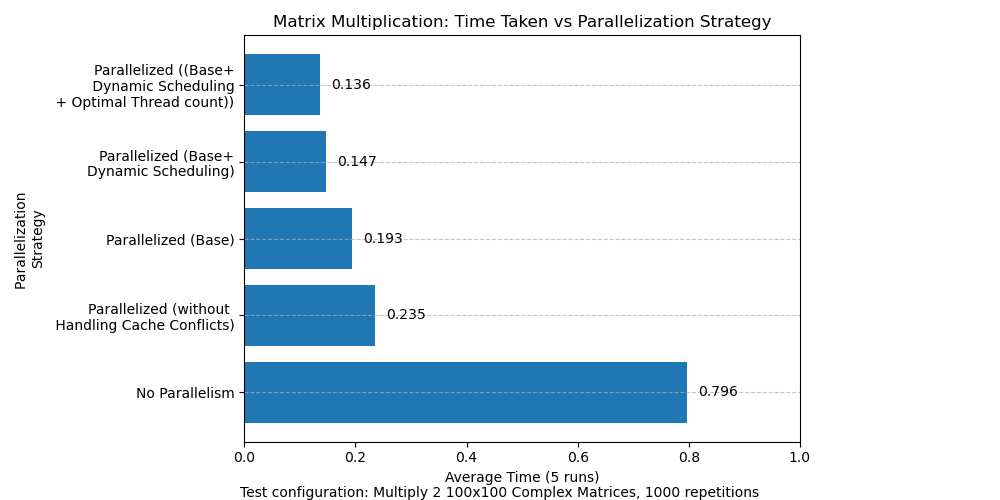
\includegraphics{matmul.png}}
% \end{figure}
\\

\resizebox*{\textwidth}{!}{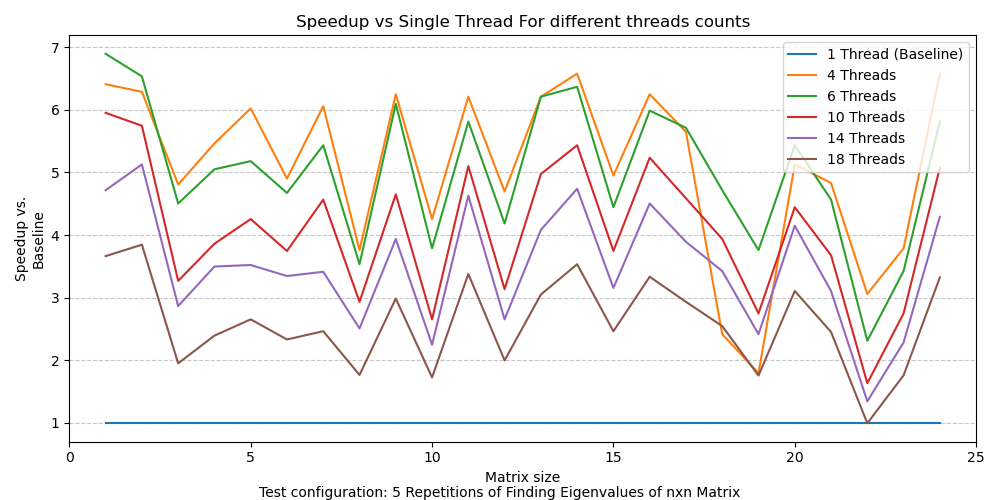
\includegraphics{threads.png}}

\bigskip

The impact of parallelization is clear. You can also see how 4 or 6 threads performs the most optimally across all loads, despite the test machine having 18 logical cores. This makes sense as it matches the number of Performance Cores on the test machine, the remaining cores were efficiency cores which were essentially a bottleneck.

\subsection{Optimizations for the QR Eigenvalue Algorithm}

There are 2 primary ways to speed up QR factorization. Deflation and Shifting
\\

Deflation essentially means identifiying certain eigenvalues that have already converged on the diagonal, and removing those rows and columns from the matrix, thus "deflating" it. This provides a very significant speedup. There are different criteria for judging the convergence of a specific eigenvalue.
\\

\resizebox*{\textwidth}{!}{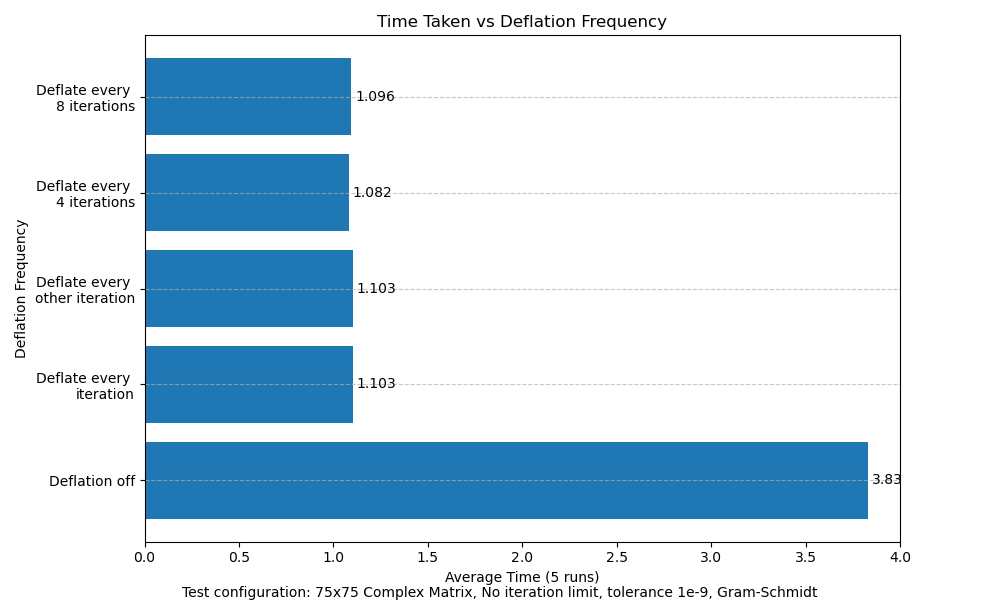
\includegraphics{deflation.png}}

\bigskip

Shifting Involves replacing $\vec{A}$ with $\vec{A} - \lambda\vec{I}$ and then later adding $\lambda$ back to the eigenvalues to shift them back. This helps shake the matrix out of certain adverserial forms (Cases with clustered up eigenvalues or Near-symmetric matrices) where it takes many iterations to converge. $\lambda$ can be chosen optimally using the Rayleigh Quotient of the matrix 
\\

\subsection{Optimizing Gram-Schmidt}

One way to parallelize Gram-Schmidt is to simply parallelize the calculations of the projections of a vector along other vectors before subtracting all those projections at once, since all previous vectors will be orthogonal anyways, one subtraction will not affect the value of a different projection. However for small matrices the overhead of parallelization may not actually be worth relatively small number of calculations as compared to those in other parts of the program such as matrix multiplication. % Graph opportunity

\subsection{Optimizing Householder}

A large part of the computational overhead of Householder comes from matrix multiplication, Which means that it is already highly optimized if we just optimize matrix multiplication. However there is also scope for optimization in the fact that subsequent reflections only affect part of the matrix, Hence if adjust our program to only perform calculations for those elements, we can skip a lot of useless computation. % Graph opportunity

\subsection{Performance Comparisons}

\resizebox{\textwidth}{!}{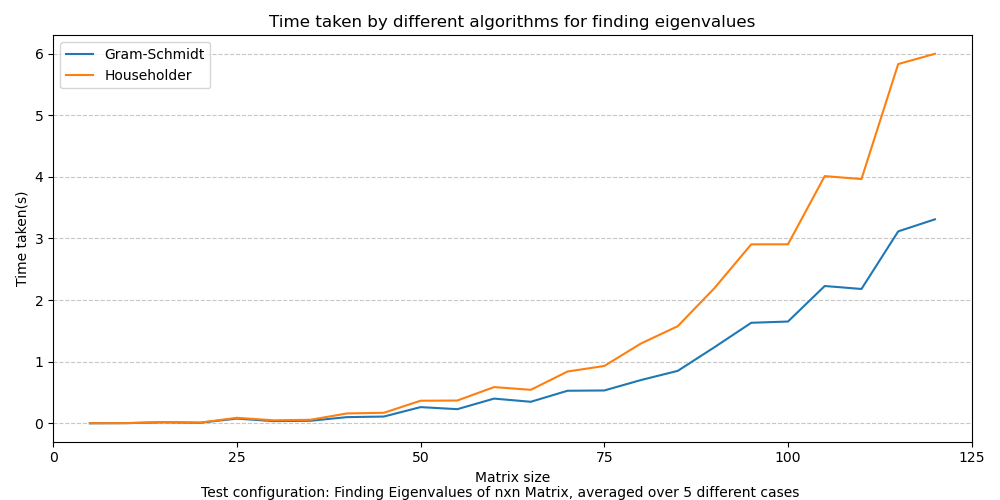
\includegraphics{algo.png}}

\bigskip

I found that both algorithms perform similarly at matrix sizes upto around 50x50, beyond which Gram-Schmitt starts outperforming Householder. This is perplexing because Householder runs for more or less the same number of QR Factorization iterations as Gram-Schmitt on each case. The reason for this becomes somewhat clear when we look at the iteration number at which deflation occurs.

Most eigenvalues deflate in the same number of iterations, independent of algorithm, but in large matrices, in the final few algorithms, the final few eigenvalues take a lot longer to converge. So it takes more iterations, and also more computation per iteration, This is the root cause of the slowdown. It is possible this might have been remedied by adding shifting however I did not have time to experiment with that.

None the less, one can see that both curves follow the same rough curvature, which confirms our previous finding that they both have the same time complexity.

\subsection{Miscellaneous Performance Gains}

Here is a list of other ways of improving performance that did not fit well into the above categories but I still want to mention:

\begin{itemize}
    \item Using the \verb|-Ofast| compiler flag in gcc improves performance greatly (This does hurt numerical stability as it breaks floating point associativity but it still gives more or less the same eigenvalues).
    
    \item Using the \verb|-mavx2 -march=native| flags to enable compiler vectorization where possible.
    
    \item Minimizing memory-related operations by smartly reusing the same memory allocation for newer matrices in the iterative approaches.
    
    \item Using macros instead of functions for minor operations increases inlining, although often times the compiler will do this automically anyways.
\end{itemize}

\section{Acknowledgements}

I would like to thank Sam Altman for his Intellectual support (through providing GPT-4o for free).
Additionally, I would like to thank IITH Library for providing access to otherwised paywlled scientific journals. 

\section{References}

\begin{enumerate}
    \item 3Blue1Brown's video lecture on Eigenvectors. \href{https://www.youtube.com/watch?v=PFDu9oVAE-g}{\texttt{https://www.youtube.com/watch?v=P\newline FDu9oVAE-g}}
    
    \item A Divide and Conquer Method for the Symmetric Tridiagonal Problem, Numerische Mathematik Vol 36. \href{https://gdz.sub.uni-goettingen.de/id/PPN362160546_0036?tify={\text22pages\%22\%3A[181]}}{https://gdz.sub.uni-goettingen.de/id/PPN362160546\_0036?tify=\newline \{\%22pages\%22\%3A[181]\}}
    
    \item Cornell Fall 2009 Notes on Householder QR \href{https://www.cs.cornell.edu/~bindel/class/cs6210-f09/lec18.pdf}{https://www.cs.cornell.edu/~bindel/class/\newline cs6210-f09/lec18.pdf}
    
    \item Physics Forums Thread: What is a Quasi Upper Triangular Matrix \href{https://www.physicsforums.com/threads/what-is-a-quasi-upper-triangular-matrix.633161/}{https://www.\newline physicsforums.com/threads/what-is-a-quasi-upper-triangular-matrix.633161/}
    
    \item Using OpenMP with C - CU Research Centre Docs \href{https://curc.readthedocs.io/en/latest/programming/OpenMP-C.html}{https://curc.readthedocs.io/en/latest/\newline programming/OpenMP-C.html}

    \item OpenMP - Scheduling, by Yiling \href{https://610yilingliu.github.io/2020/07/15/ScheduleinOpenMP/}{https://610yilingliu.github.io/2020/07/15/Schedulein\newline OpenMP/}

    \item An Efficient Eigensolution Method and Its
    Implementation for Large Structural Systems \href{https://repositories.lib.utexas.edu/items/af4761cd-de0d-451f-ac02-d10becb0ae28}{https://repositories.lib.utexas.edu/items/af4761cd-de0d-451f-ac02-d10becb0ae28}
\end{enumerate}
% 3B1B
% Wikipedia
% IITH library for journal access
% That journal on Divide and Conquer
% LAPACK Docs
% Valgrind
% Cornell Pseudocode

\end{document}
